% Lablog fixture: diagramas tipo Feynman con TikZ puro (XeTeX/Tectonic)
% No depende de tikz-feynman (Lua). Live preview → bloque PDF-only.

\section*{QED: dispersión $e^-e^- \to e^-e^-$ (árbol)}
\begin{center}
\begin{tikzpicture}[
  baseline=(current bounding box.center),
  fermion/.style={thick, postaction={decorate},
    decoration={markings, mark=at position 0.55 with {\arrow{stealth}}}},
  photon/.style={decorate, decoration={snake, amplitude=1.2pt, segment length=5pt}, thick},
  every node/.style={font=\small}
]
  % leg 1 in
  \draw[fermion] (-2.2,1.2) -- (-0.6,0.3);
  \node[left] at (-2.2,1.2) {$e^-$};
  % leg 2 in
  \draw[fermion] (-2.2,-1.2) -- (-0.6,-0.3);
  \node[left] at (-2.2,-1.2) {$e^-$};
  % photon
  \draw[photon] (-0.6,0.3) -- (0.6,-0.3);
  \node[above] at (0.0,0.15) {$\gamma$};
  % leg 1 out
  \draw[fermion] (0.6,-0.3) -- (2.2,-1.2);
  \node[right] at (2.2,-1.2) {$e^-$};
  % leg 2 out
  \draw[fermion] (0.6,0.3) -- (2.2,1.2);
  \node[right] at (2.2,1.2) {$e^-$};
  % vertices
  \fill (-0.6,0.3) circle (1.6pt);
  \fill (0.6,-0.3) circle (1.6pt);
\end{tikzpicture}
\end{center}

\section*{Decaimiento $Z \to f\bar{f}$}
\begin{center}
\begin{tikzpicture}[
  fermion/.style={thick, postaction={decorate},
    decoration={markings, mark=at position 0.55 with {\arrow{stealth}}}},
  boson/.style={thick, dashed},
  every node/.style={font=\small}
]
  \draw[boson] (-2.0,0) -- (0,0);
  \node[left] at (-2.0,0) {$Z$};
  \fill (0,0) circle (1.8pt);
  \draw[fermion] (0,0) -- (1.8,1.0);
  \node[right] at (1.8,1.0) {$f$};
  \draw[fermion] (1.8,-1.0) -- (0,0);
  \node[right] at (1.8,-1.0) {$\bar{f}$};
\end{tikzpicture}
\end{center}

\section*{Loop simple (self-energy)}
\begin{center}
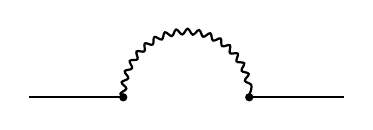
\begin{tikzpicture}[
  fermion/.style={thick},
  photon/.style={decorate, decoration={snake, amplitude=1pt, segment length=4pt}, thick}
]
  \draw[fermion] (-2,0) -- (-0.8,0);
  \draw[fermion] (0.8,0) -- (2,0);
  \draw[photon] (-0.8,0) arc (180:0:0.8);
  \fill (-0.8,0) circle (1.5pt);
  \fill (0.8,0) circle (1.5pt);
\end{tikzpicture}
\end{center}
